\documentclass[11pt]{article}
\usepackage[margin=1.1in]{geometry}
\usepackage{usefulsymbols}
\usepackage{hyperref}
\usepackage{listings}
\usepackage{courier}

%% user defined cmd
\newcommand{\kbp}{{\bf{TAC KBP}}}
\newcommand{\seml}{SemLinker}
\newcommand{\semk}{Semkit}
\def\version{{\tt 1.0.0}}
%%
\lstset{basicstyle=\small\ttfamily\color{blue},breaklines=true,frame=L,xleftmargin=\parindent}
%\lstset{framextopmargin=50pt,frame=bottomline}
%\lstset{breaklines=true} 
%\lstset{breakatwhitespace=true} 

% if you just need a simple heading
% Usage:
%   \heading{the text of the heading}
\newcommand{\heading}[1]{
    \vspace{0.3cm} \noindent \textbf{#1} \newline
}

\usepackage{relsize}
\renewcommand*{\UrlFont}{\ttfamily\smaller\relax}

\usepackage{datetime}
\newdateformat{mydate}{\monthname[\THEMONTH] \THEYEAR}


\graphicspath{{./graphics/}}

\begin{document}

\title{\textbf{\seml{}} ~ \version \\~\\~\\User Guide\\~\\~\\~\url{https://code.google.com/p/semlinker/}\\~\\~}

\author{Eric Charton\\~\\Marie-Jean Meurs\\~\\Ludovic Jean-Louis\\~\\Michel Gagnon\\~\\~\\~\\~\\~}

\date{\mydate\today}

\maketitle

% \begin{center}
% 	\includegraphics[width=0.2\textwidth]{genomicslogogreen}$\qquad$\includegraphics[width=0.2\textwidth]{genozymeslogo}$\qquad$\includegraphics[width=0.25\textwidth]{concordialogo}\\
% \end{center}

\thispagestyle{empty}
% 
\pagebreak
\tableofcontents

% \pagestyle{empty}
\thispagestyle{empty}

~\\~\\~\\
Support note: SemLinker is a powerful but complex software, documented according to normal standards (Java doc, this doc, academic papers), but not easy to use or understand. 
There are many NLP concepts and a complex evaluation framework to handle for deploying this package. 
The authors will do their best to answer questions according to their role in the development (see section 4), but no guarantee can be given that it will be enough to help ones to deploy this system.
\pagebreak

\section{Overview}
\label{sec:overwiew}

\seml{} is a Java library designed to experiment various applications of text mining and annotations. 
Using an external annotator (currently \url{www.wikimeta.com}), \seml{} can apply various annotation layers and information extraction processes on a text document. 
\seml{} is divided in two main components: 
\begin{enumerate}
 \item the \textbf{\semk{}} component
 \item the \textbf{KBP} component
\end{enumerate}

\subsection{\semk{}}
\label{ssec:semk}
\semk{} is a set of classes and demos dedicated to apply annotation layers on a text document. 
Those annotation layers can be Part Of Speech tags, Named Entity labels, Semantic Links. 
\semk{} also includes a Natural Language Processing set of classes intended to manage specific linguistic phenomenons like co-references. 
\semk{} produces an \underline{annotation object} from a text document using an annotation engine. \semk{} is used in the KBP experimental component.

\subsection{KBP component}
\label{ssec:kbpcomp}
This component is an experimental platform compatible with the NIST TAC-KBP\footnote{\url{http://www.nist.gov/tac/2013/KBP/}} entity linking task. 
The goal of TAC Knowledge Base Population (KBP) is to develop and evaluate technologies for building and populating knowledge bases (KBs) about named entities from unstructured text. KBP systems must either populate an existing reference KB, or else build a KB from scratch. 

\subsection{Configuration}
\label{ssec:config}

\subsubsection{Software requirements}
\label{sssec:softreqs}
You need:
\begin{itemize}
 \item a true Java 7 compliant VM. We recommand the Oracle one: \url{http://www.oracle.com/technetwork/java/javase/downloads/index.html} 
 \item a version of the NLGbAse metadata (one is in the metadata folder of the \seml{} library): \url{http://www.nlgbase.org} 
 \item a semantic annotation API key (free for academics): \url{http://wikimeta.org/product_api.html}
\end{itemize}

\subsubsection{Optional requirements}
\label{sssec:optreqs}
\begin{itemize}
 \item You need to install the Redis Base, available for Linux and Windows: \url{http://redis.io/download}
 \item You might need various resources to reproduce the KBP task (see KBP section)
\end{itemize}

\subsubsection{System requirements}
\label{sssec:sysreqs}
Most of the calculation requirements are handled by the external API. 
A classical computer with the following properties will be suitable:
\begin{itemize}
 \item Centrino / AMD FX / Athlon
 \item 2 cores
 \item 8 GB RAM
 \item 500 GB Hard Drive
 \item Internet access (classical ADSL bW)
 \end{itemize}

\noindent Note: the memory size will be the most important part of a \seml{} workstation. 
Less than 8 GB can lead to swap activation and loss of PC usability. 

\subsubsection{Configuration file}
\label{sssec:cfg}
When everything is installed you need to configure \textit{config.cfg} file according to the folders of your system. 
The \textit{config.cfg} file must be in the same folder as the \seml{} JAR file or in the root folder of \seml{} if you use eclipse to launch it.\\
\\
\underline{For \seml{} global configuration please set}:\\
\\
wmresturi=uri\_of\_your\_API\_rest\_interface\\
apiaccount=key\_numer\_of\_your\_API\_Account\\
\\
To obtain those information, please open a free API account on Wikimeta:

\begin{center}
  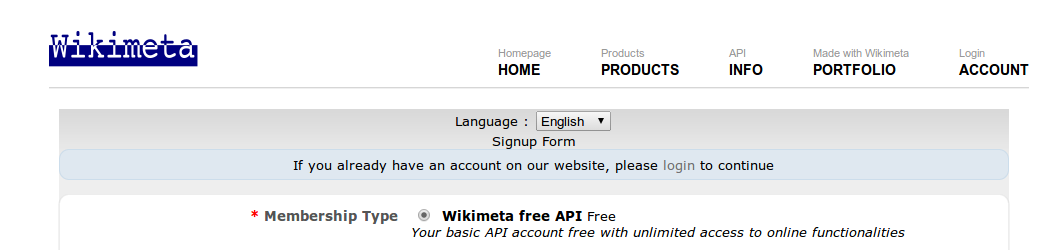
\includegraphics[width=\textwidth]{wikimeta_account}\\
\end{center}

\noindent Then collect the information of the API on your user interface. 
See next page illustration to view how to collect your API information in the Wikimeta user Interface. \\
\\
By default, \seml{} is configured with an anonymous Demo account, we cannot guarantee that this account will remain open. 
Please note that unlimited API accounts will be provided to academic users for experimental purposes. 
To activate your unlimited API account, just send a mail to contact@wikimeta.com using your academic email address and giving your Wikimeta account reference. 


\begin{center}
  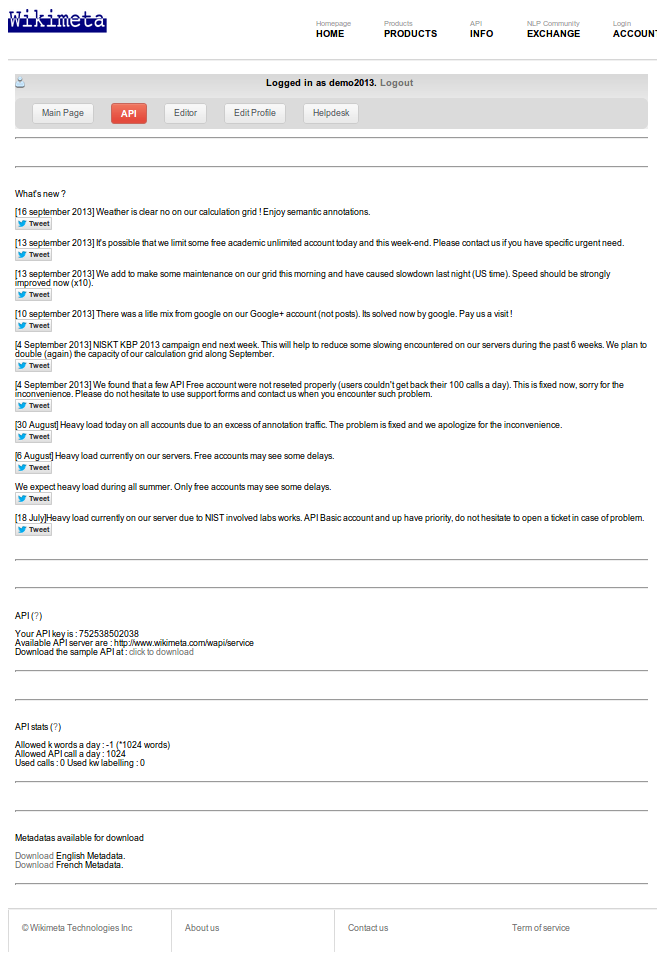
\includegraphics[width=\textwidth]{wikimeta_api}\\
\end{center}

\noindent\underline{For KBP module configuration, please check \textit{config.file}, and set}:\\
\\
\texttt{HOME\_DIR=/\textbf{YOUR\_PROJECT\_HOME\_PATH}/SemLinker/}\\
\texttt{INDEX=/\textbf{YOUR\_PATH\_TO\_LUCENE\_INDEX\_OF\_KBP\_CORPORA}/index\_kbp\_folder}\\
\texttt{INDEX\_WIKIPEDIA=/\textbf{YOUR\_PATH\_TO\_INDEXED\_WIKIPEDIA}/indexwiki\_folder}\\
\texttt{NLGBASE\_PATH=\textbf{YOUR\_PATH\_TO\_METADATA}/metadata/EN.data.csv}\\
\\
If you mount \seml{} as an eclipse project, \texttt{\textbf{YOUR\_PATH}} will be usually to your eclipse workspace.
Information on those parameters and the related resources are given in section~\ref{ssec:kbpreqs}.


\subsubsection{Loading a Redis Base of NLGbAse metadata}
\label{sssec:redisdb}
Some applications of \seml{} need to access to a Redis Base (NoSQL database) to collect the NLGbAse metadata. \\
Follow this process to prepare this Redis Base:
\begin{enumerate}
 \item Download and install a Redis Server on your system (Redis is free)
 \item Launch the server (usually ./redis-server in the folder src after compilation)
 \item Verify that the config file section nlgbasepath of \seml{} is pointing on\\{semlinker\_folder}/metadata/EN.data.csv
 \item Load the base with the command \texttt{\textcolor{blue}{java -cp semlinker.jar Tool}}
\end{enumerate}

\noindent Watch the base loading. 
After a long process (many hours) That’s all.\\
Next time you do not need to reload the Redis Base, but just to start the server.


%%%%%%%%%%%%%%%%%%%%%%%%%%%%%%%%%%%%%%%%%%%%%%%%
\section{\semk{}}
\label{sec:semk}

There is no specific requirements for usage of the \semk{} application for text annotation using the demo classes. 

\subsection{Demos}
\label{ssec:demos}
The demo classes are intended to present some short sequences of code that demonstrate a possibility of the \seml{} library. 
Please refer to the JavaDoc for all the specific commands of \semk{} demos.

\subsubsection{ApiCallSample}
\label{sssec:apicall}
Make a call to the API according to the configuration file and return the annotation. 
\begin{lstlisting}
java -cp semlinker.jar semkit.demos.ApiCallSample  -text text.txt
\end{lstlisting}
The options are as follows:
\begin{lstlisting}
-h help
-apikey key / define your own API key
-text filename / annotate a text file given in command line
-distrib / display the word distribution
-decodejson / display the JSON decoding
-language {EN|FR} / force a language of annotation
\end{lstlisting}

\subsubsection{BuildHTMLSample demo}
\label{sssec:buildhtml}
A class that demonstrates how to annotate a document, refine it, and then transform it in HTML code for a website. 
\begin{lstlisting}
java -cp semlinker.jar semkit.demos.BuildHtmlSample -text text.txt
\end{lstlisting}

\subsubsection{SemanticExtractorSample}
\label{sssec:semextr}
Give it a text with name of political people and it returns their affiliation, birthdate and birthplace like this:
\begin{lstlisting}
java -cp semlinker.jar semkit.demos.SemanticExtractorSample -text text.txt
\end{lstlisting}
The output is as follows:
\begin{lstlisting}
EN: Pierre Moscovici (LOD :http://www.dbpedia.org/resource/Pierre_Moscovici  ) 
-Document returned ok 
      ->Political affiliation of Pierre Moscovici is http://dbpedia.org/resource/Socialist_Party_(France) 
      ->Birthdate of Pierre Moscovici is 1957-09-16"^^<http://www.w3.org/2001/XMLSchema#date 
\end{lstlisting}



\subsection{How to build and manage an annotation object}
\label{ssec:annotobj}
The principle of annotation objects allows you to annotate a document and then to apply various processes to the object representing this document.

\subsubsection{Create an annotation object}
\label{sssec:creatannobj}
There is a full example of all those processes in the BuildHTMLSample class:\\
\\
\underline{First annotate a document using the API}:\\
\begin{lstlisting}
// Wikimeta Extractor 
result = WikiMetaExtractor.getResult(  SemanticConstants.APIAccount , WikiMetaExtractor.Format.XML, toannotate , ln);
\end{lstlisting}

\noindent\textit{String result} is the resulting annotation in RAW XML of the \textit{String toannotate}.\\
\\
\underline{Build an annotation object}:\\
\begin{lstlisting}
// Wikimeta decoder
WikiMetaXMLDecoder annotations = new WikiMetaXMLDecoder(result, 15);
\end{lstlisting}

\noindent\textit{annotations} is the annotation object resulting of the \noindent\textit{String result} raw XML file.\\
\\
\underline{You can now access this object properties as follows}:\\
\begin{itemize}
 \item \textbf{int annotations.size()} is the number of lines in the object. Each line contain a unique word or symbol (commas, sent separator and so on)
 \item \textbf{String word = annotations.getwordatpos(int x)}: get the word at a x given position.
 \item \textbf{String namedentity = annotations.getENLabel(int x)}: get a named entity tag at given position if exists or null
\end{itemize}
\textit{See the Javadoc for WikimetaXMLDecoder for all the available method (collecting surface form, part of speech tag and so on)}




\subsubsection{Normalize annotation objects}
It is possible to \textbf{improve the accuracy of annotation} using the whole document content. 
This is the normalization process using co-reference and named entity normalization (see the KBP 2013 system paper for more information). \\

\textbf{Apply co-reference normalization to an annotation object.}
\begin{lstlisting}
 // re-apply coreferences corrections after NE Normalizer
annotations = SimpleCoreferenceDetector.applyCoreferenceCorrection(annotations);
\end{lstlisting}

\textbf{Apply Named Entity normalization to an annotation object.}
\begin{lstlisting}
NormalizeNE NEnorm = new NormalizeNE();

// apply NE normalizer
annotations = NEnorm.rerankNE(annotations);
\end{lstlisting}

\textbf{Apply mutual disambiguisation to an annotation object.}
\begin{lstlisting}
MutualDisambiguation mdiz = new MutualDisambiguation();

// Disambiguate using document mutual relations
annotations = mdiz.disambig(annotations, content);
\end{lstlisting}

\textit{String Content} is the original text document.

%%%%%%%%%%%%%%%%%%%%%%%%%%%%%%%%%%%%%%%%%%%%%%%%%%%%%%%%%%%%%%%

\section{KBP}
\label{sec:kbpcamp}
KBP is an international evaluation campaign organized by the NIST administration in the context of TAC conferences. 
KBP can be decomposed into two complementary tracks: 
entity linking, in which entity mentions must be aligned with entities in the reference Knowledge Base (KB) or new entities discovered in the document collection; 
and slot filling, which involves finding predefined attributes about target entities in unstructured text. 
A third major KBP track is Cold Start KBP, which combines entity linking and slot filling to populate an empty KB using the predefined schema from slot filling. 
We include in the \seml{} toolkit a complete platform to reproduce a KBP entity linking experiment. 

\subsection{KBP component requirements}
\label{ssec:kbpreqs}
The \seml{} KBP component needs a set of resources to work properly. 
Some of those resources are free to use, others are subject to specific copyright and distribution restrictions (like the evaluation corpora from LDC). 
The following components are mandatory to build a complete NIST KBP experiment:
\begin{enumerate}
 \item Lucene Indexed KBP corpora
 \item KB correspondence table
 \item Lucene indexed Wikipedia XML dump (English)
 \item Optional: Lucene Search for Wiki (this can be replaced by a direct access to Wikipedia search engine)
\end{enumerate}

\subsubsection{KBP corpora}
\label{sssec:kbpcorp}
As explained on the NIST KBP website access to KBP corpora is restricted to KBP task participants:\\
\textit{``Data that are required for the TAC KBP 2013 tracks are distributed at no cost to track participants. 
Whenever possible, data are distributed by NIST or the Linguistic Data Consortium via Web download; 
data are mailed as physical disks only if they cannot be made available for download. 
Access to TAC KBP 2013 data is restricted to registered TAC KBP 2013 participants who have submitted all the required User Agreement forms. 
Each participating team will provide a TAC KBP 2013 Team ID and will receive a Team Password upon registration. 
Teams that have participated in past TAC cycles must register and obtain a new TAC KBP 2013 Team ID and password for 2013.''}\footnote{Text from \url{http://www.nist.gov/tac/2013/KBP/data.html}}

Once the corpus obtained from LDC as KBP participant or ordered, you can index it for \seml{} with Lucene using the class (\textbf{if config file is properly configured}):
\begin{lstlisting}
kbp2013.index.indexSourceCorpus
\end{lstlisting}
Or with the command line :
\begin{lstlisting}
java -cp semlinker.jar kbp2013.index.indexSourceCorpus
\end{lstlisting}

\subsubsection{Reference KB and correspondence table}
\label{sssec:refkb}
The reference KB for 2013 is based on a snapshot of English Wikipedia from October 2008 and is the same reference KB that has been used in TAC KBP since 2009. 
Each node in the reference KB corresponds to a Wikipedia page for a person (PER), organization (ORG), or geopolitical entity (GPE), 
and consists of predefined attributes (a.k.a "slots") derived from Wikipedia infoboxes. 
Unstructured text from the Wikipedia page is also available (as "wiki\_text") in the reference KB. 

As \seml{} uses external annotations engine to solve the entity linking task, the Wikipedia links provided have to be compliant with the KB nodes numbering system. 
A correspondence table is generated using NLGbAse (see TAC KBP conference paper for details) with this class :
\begin{lstlisting}
kbp2013.tools.buildKBTable
\end{lstlisting}

Caution: to use this class, you need to have a Redis Base loaded with the NLGbAse corpus on your computer (see 1.c.iv).

\textbf{Note}: You do not need to regenerate the correspondence table until you want to use the latest NLGbAse version. 
A pre-calculated sample of the correspondence table is present in folder: \textit{resources/kbp2013/wikimeta\_table}


\subsubsection{Wikipedia dump indexation}
\label{sssec:wikipdumpindx}
To use the mutual disambiguation capabilities of \seml{}, you need to index a full dump of an English Wikipedia. 
This is done using the class (\textbf{if config file is properly configured}):
\begin{lstlisting}
kbp2013.index.indexWikipediaCorpus
\end{lstlisting}
Or with the command line:
\begin{lstlisting}
java -cp semlinker.jar kbp2013.index.indexWikipediaCorpus
\end{lstlisting}

\textbf{Note}: if you do not build a Wikipedia Dump index with Lucene, \seml{} will try to collect the Wikipedia page directly online using the Wikipedia API. 
This has a strong impact on the speed of the experimental process (over 10 times longer to process all the experiments of KBP2013 test queries). 
We do not recommend you to use this option.

\subsubsection{Lucene-Search for Wiki}
\label{sssec:lucsrch}
\textbf{Note}: installing Lucene-Search for Wiki can be complex and difficult, and involves a lot computing resources. 
By default, \seml{} includes a hack that access directly to the \textit{``Did You Mean''} page of Wikipedia (see Figure~\ref{fig:didumean}) rather than invoke a local copy of Lucene-Search for Wiki. 

This solution avoids the need of time consuming configuration, and offers nearly the same results as these obtained with a local copy. 

\begin{figure}
\begin{center}
  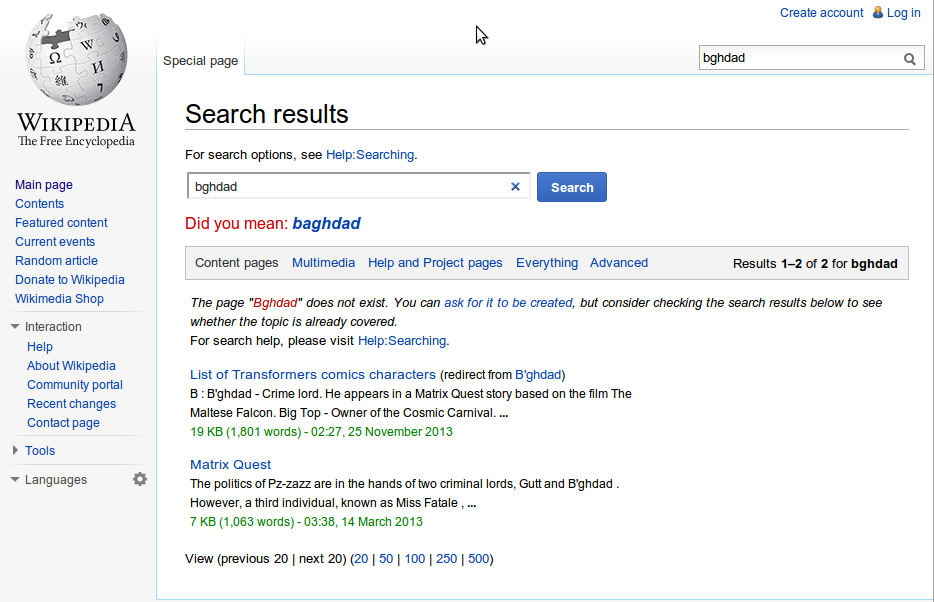
\includegraphics[width=\textwidth]{wikipedia_didumean}
  \caption{Wikipedia ``Did you mean'' page}
  \label{fig:didumean}
\end{center}
\end{figure}

\subsection{Experiment}
Once the complete system is configured and ready to operate, configure properly the path in the config file to the query file and launch:
\begin{lstlisting}
kbp2013.LinkEntities
\end{lstlisting}

That's all! You see all the experiments rolling for each query.\\

The generated file is output in your \texttt{TEST\_DIR} folder defined in config file and is directly compliant with the KBP evaluation script. \\

We included this script (el\_scorer.py)in the folder:\\
\texttt{resources/kbp2013/entitylinkingeval/scripts}\\
\\
We also included a modified version of this script (\texttt{el\_scorer\_seg.py})in the folder to allow calculation of score for each component of the KBP task 
(for example a specific score per named entity, per sub corpus...).


\section{Credits}
\label{sec:credits}

\subsection*{Redaction of this version of the document}
\begin{itemize}
 \item[] Eric Charton, \'{E}cole Polytechnique de Montr\'eal [\texttt{{\small{eric.charton@polymtl.ca}}}]
 \end{itemize}


\subsection*{Contributors on the \seml{} code V\version}

\begin{itemize}
 \item[] Eric Charton, [\texttt{{\small{eric.charton@polymtl.ca}}}]\\ 
	Main Architect, worked  on almost all classes :-)\\

\item[] Marie-Jean Meurs, [\texttt{{\small{marie-jean.meurs@concordia.ca}}}]\\
	Normalization, query reformulation, worked on various classes, cleaning, and refactoring.\\

\item[] Ludovic Jean-Louis, [\texttt{{\small{ludovic.jean-louis@polymtl.ca}}}]\\ 
	Indexation, worked on various classes and main author of KBP corpus and Wikipedia indexation classes.\\

\item[] Michel Gagnon, [\texttt{{\small{michel.gagnon@polymtl.ca}}}]\\
	Engineering, normalization, and refactoring
\end{itemize}

\section{Complementary informations}
\label{sec:compinfo}
The technical description of the \seml{} system presented in KBP 2013 evaluation campaign is in this paper:\\
\\
Eric Charton, Marie-Jean Meurs, Ludovic Jean-Louis, Michel Gagnon,\\
\textit{SemLinker system for KBP2013: A disambiguation algorithm based on mutual relations of semantic annotations inside a document.}\\
Proceedings of TAC KBP 2013\\
\\
Javadoc:


% Contact information can be found at \url{}.

% \appendix

% \bibliographystyle{acm}
% \renewcommand{\baselinestretch}{0.0}
% \bibliography{usermanual}

\end{document}
